% Diagrama 4: componentes de un mosaico SAR (Liu et al., 2024) y cómo los cubre este flujo
% Compila en Overleaf con pdfLaTeX o XeLaTeX.
\documentclass[border=12pt]{standalone}
\usepackage{iftex}
\ifPDFTeX
  \usepackage[utf8]{inputenc}
  \usepackage[T1]{fontenc}
  \usepackage[scaled]{helvet}
\else
  \usepackage{fontspec}
  \setsansfont{texgyreheros}[Extension=.otf, UprightFont=*-regular,
    BoldFont=*-bold, ItalicFont=*-italic, BoldItalicFont=*-bolditalic, Scale=0.95]
\fi
\renewcommand{\familydefault}{\sfdefault}
\usepackage{tikz}
\usetikzlibrary{arrows.meta, positioning}

\definecolor{azul}{HTML}{1F5A96}
\definecolor{verde}{HTML}{2E7D32}
\definecolor{naranja}{HTML}{E07B00}
\definecolor{gris}{HTML}{455A64}

\begin{document}
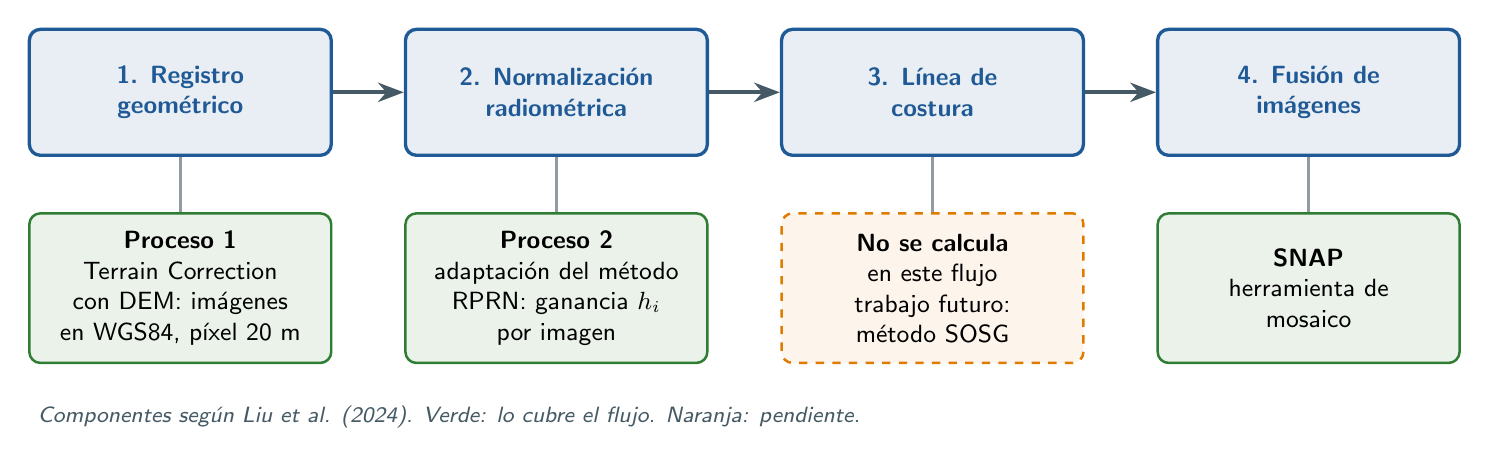
\begin{tikzpicture}[
  >=Stealth,
  comp/.style={rectangle, rounded corners=4pt, draw=azul, line width=1.2pt,
               fill=azul!10, text width=3.6cm, minimum height=1.6cm,
               align=flush center, font=\small\bfseries, text=azul},
  si/.style={rectangle, rounded corners=4pt, draw=verde, line width=0.9pt,
             fill=verde!10, text width=3.6cm, minimum height=1.9cm,
             align=flush center, font=\small},
  no/.style={rectangle, rounded corners=4pt, draw=naranja, dashed, line width=0.9pt,
             fill=naranja!8, text width=3.6cm, minimum height=1.9cm,
             align=flush center, font=\small},
  flecha/.style={->, line width=1.4pt, draw=gris},
  enlace/.style={line width=0.9pt, draw=gris!60}
]

\node[comp] (c1) {1. Registro\\ geométrico};
\node[comp, right=9mm of c1] (c2) {2. Normalización\\ radiométrica};
\node[comp, right=9mm of c2] (c3) {3. Línea de\\ costura};
\node[comp, right=9mm of c3] (c4) {4. Fusión de\\ imágenes};

\foreach \a/\b in {c1/c2, c2/c3, c3/c4}
  \draw[flecha] (\a.east) -- (\b.west);

\node[si, below=7mm of c1] (e1) {\textbf{Proceso 1}\\ Terrain Correction\\ con DEM: imágenes\\ en WGS84, píxel 20~m};
\node[si, below=7mm of c2] (e2) {\textbf{Proceso 2}\\ adaptación del método\\ RPRN: ganancia $h_i$\\ por imagen};
\node[no, below=7mm of c3] (e3) {\textbf{No se calcula}\\ en este flujo\\ trabajo futuro:\\ método SOSG};
\node[si, below=7mm of c4] (e4) {\textbf{SNAP}\\ herramienta de\\ mosaico};

\foreach \a/\b in {c1/e1, c2/e2, c3/e3, c4/e4}
  \draw[enlace] (\a.south) -- (\b.north);

\node[font=\footnotesize\itshape, text=gris, anchor=north west]
  at ([yshift=-4mm]e1.south west)
  {Componentes según Liu et al. (2024). Verde: lo cubre el flujo. Naranja: pendiente.};

\end{tikzpicture}
\end{document}
